\documentclass[10pt,a4paper]{article}
\usepackage[utf8]{inputenc}
\usepackage{amsmath}
\usepackage{amsfonts}
\usepackage{amssymb}
\usepackage{graphicx}
\title{CROAC: Counting and Recognition using Omnidirectional Acoustic Capture}
\author{Marcel Gietzmann-Sanders}
\begin{document}
\maketitle
\tableofcontents
\newpage
\section{The Pond}
It's an hour past sunset and the rain has just subsided. I approach the pond - a vernal pool that will dry up sometime this summer - trying as best I can to be a ghost. Unfortunately the crinkling of leaves reveals my corporeality and a hush descends upon the pond. It is as if the frogs recognize that their rehearsal time is over and have gone backstage in a mist of whispers as they let me get seated in anticipation of the grand event. Groping about in the darkness, as I have put out my head torch, I find the most comfortable seat in the house - a patch of dirt nestled among the roots of an old maple tree - and settle in. On the walk of mile or so in I've already heard the spring peepers chirping in all their eagerness and bullfrogs announcing their grandiose dominion with their earthly croaks, but I know that was all but a taste of what is to come. So I settle back  and wait for the concert to start.

It begins with solitary croaks as the bolder of the frogs begin to test the air, seeing whether their audience still stirs. But soon enough their comrades join in and the sound begins to mount. Layer by layer I hear different species enter the ensemble. Region by region the pond gets louder and louder as the frogs regain their composure. Before I know it the air is so thick with sound I feel as if I could breath it in. 

In full chorus it is impossible for me to discern the individual voices that make up this extraordinary orchestra. Instead all my two ears receive is a wall of frenetic sound. Yet the physicist in me recognizes this as a mere illusion and as I sit there bathed in chirps and croaks and wheezes I relish the richness of the data before me. I know that what my ears hear as a single curtain is in fact a richly woven fabric of pitches, amplitudes, and phases - a mathematical puzzle waiting to be untangled and solved. I realize that every spring night, and many a summer one too, these frogs broadcast into the ether a whole host of information on position, counts, energy, species, and perhaps even lineage. All waiting to be deciphered by a discerning soul. And so as I sat there at the base of that maple tree, bathed in the ciphered data of my amphibian friends, I wondered what it would take to break the code of frogs. The adventure into mathematics, computation, and herpetology that ensued has brought me untold joy, and I hope that in the subsequent paragraphs I can give you little taste of that adventure too. 
\newpage
\section{The Richness of Sound}
We begin with a picture - specifically Figure 1. This is nothing more than a picture of the simplest wave possible. If you've ever plucked a guitar string you'll know that sound is the result of vibrations. When some object like a string, or a speaker, or your very own vocal chords vibrate that vibration translates into waves in the air which we then hear as sound. Given that all sound is composed of waves like these, we can begin our journey in trying to differentiate different sound sources by understanding what makes one wave different from the next. And an excellent way to do this is to look to the richest source of sound that our ears already find intelligible - music. 

\begin{figure}[!htb]
\center{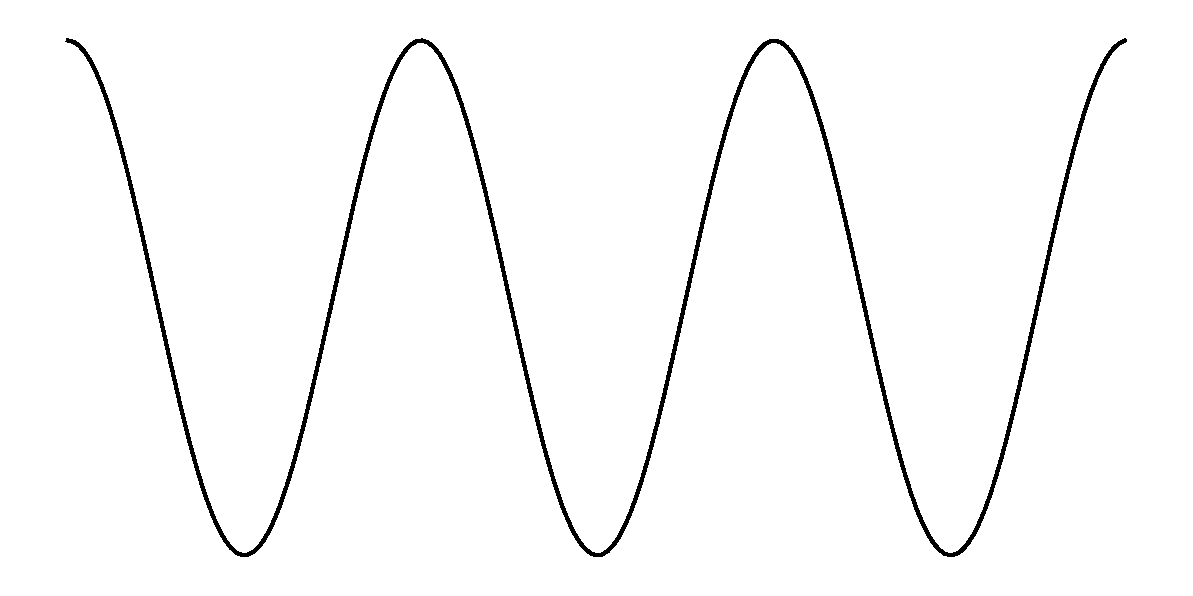
\includegraphics[width=\textwidth]
{figures/a_basic_wave.pdf}}
\caption{\label{fig:my-label} A Simple Wave}
\end{figure}

\subsection{Blue Whales Yelling - Amplitude}
What makes music such a great place to start is the fact that the human mind is already so used to picking out different sections, rhythms, and instruments - an activity quite similar to what we want to do with our frog chorus. When you go to a concert you can distinguish the vocals from the percussion, and the harmony from the melody. But, depending on the kind of concert it can be much more difficult picking out what your friends are trying to say when you're already having to yell to hear yourself. And by the end you'll all be speaking in muted whispers no matter how loud you try to speak because you'll have lost your voices half way through the performance. This contrast, conveniently, is our first and simplest discriminator of sound - volume. As you raise your voice the volume of the sound that you are producing increases. The fact that you can barely hear each other speaks to the enormous volume of sound coming from the stage. So how is this represented in our wave? Volume is determined by the height of our wave - the farther the undulation has to go between each peak and valley the louder the sound is. This height is referred to as the \textbf{amplitude} and to get a sense of just how variable amplitude can be let's bring a blue whale to the concert.

Blue whales are the largest animals to have ever lived. Rather unsurprisingly then, they can be rather loud. How loud? Well let's just say that blue whales would have no trouble hearing each other at a rock concert. In fact they may instead draw the ire of their fellow concert goers as they drown out the music with their voices. The typical sound level at a rock concert is around 110 decibels (dB) \cite{chris}. Blue whales on the other hand have been recorded at up to 180 dB \cite{zcormier}. This difference is actually far more ridiculous than it first seems because of what a decibel actually is. When a decibel measurement increases by 10 it means the sound is around 3 \textit{times} louder. All to say that if our blue whales raised their voices, their chatter could get up to 21 times louder than the rock concert! Quite rude. Graphing this out in Figure 2 we can see that the amplitude of the blue whales yelling at one another (dashed line) is so large in comparison to the amplitude of the rock concert (solid line) that the rock concert's sound barely looks like a wave at all. Pretty incredible.

\begin{figure}[!htb]
\center{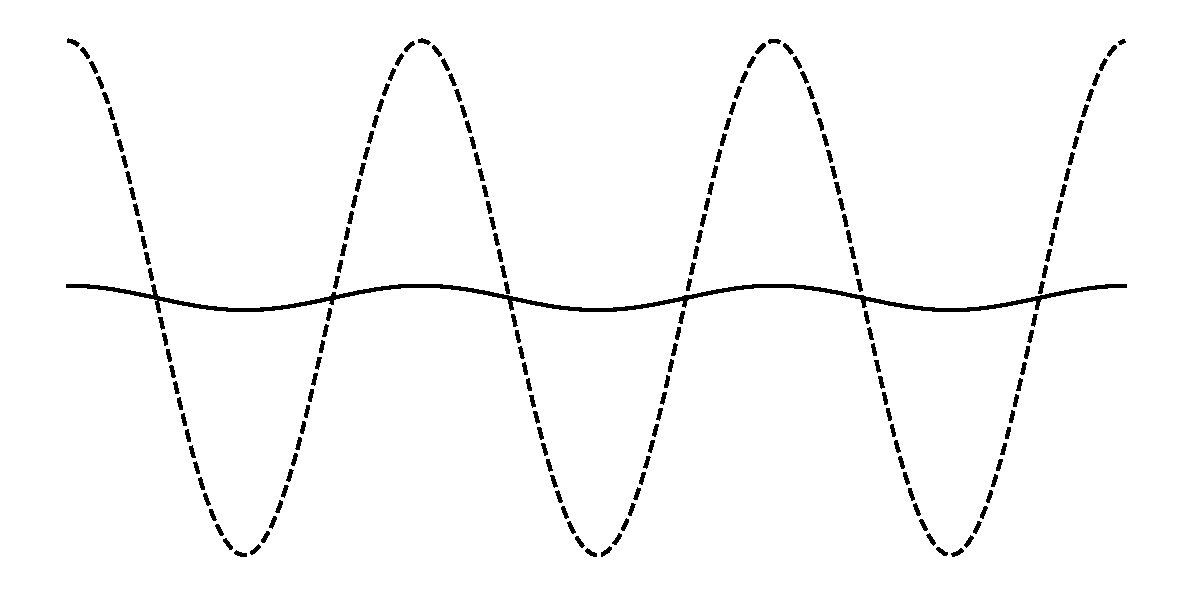
\includegraphics[width=\textwidth]
{figures/blue_whale_comparison.pdf}}
\caption{\label{fig:my-label} Blue Whale v. Rock Concert}
\end{figure}

\subsection{To Tune or Not to Tune - Pitch}
Okay, so amplitude is one way to distinguish one wave from another - what's up next? Well let's stop worrying about hearing our friends for a moment and turn back to the music. Remember how we said it's pretty easy for our brains to distinguish the vocalists from, say, the bass? Well there's a good reason for that - pitch. Pitch is how high or low a sound sounds. When that bass is rumbling all through your body you're experiencing a sound with a very low pitch. On the other hand when the singer hits that high note with a full crescendo that's a sound with an exhilarating high pitch. How does pitch show up in our wave? Well in contrast to amplitude - which was how high our waves got - pitch is all about how wide they are. The distance from one peak to the next is called the \textbf{wavelength} and the larger that distance is the lower the pitch of the sound. Pitch however is rarely measured in wavelengths. Instead the standard measurement used is something called Hertz (Hz). Hertz is a unit of \textbf{frequency} and frequency is simply the number of complete oscillations (peaks and troughs) per unit time. So, for example, when you hear that orchestras tune to A440 that 440 is specifically 440 Hz. Frequency and wavelength are interchangeable and tied together by a simple formula. Using the fact that we know the speed of sound $c$, if $w$ is the wavelength and $k$ is the frequency then the conversion is simply:

\begin{equation}
w = c/k
\end{equation}

So for example, if the speed of sound is 343 meters per second (m/s) then the wavelength of A440 is $343/440\approx0.78m$ or just over 2.5 feet. In comparison the highest note on a typical piano is at 7900 Hz \cite{wikipiano} which corresponds to a \textit{much} smaller wavelength ($343/7900=0.04m$). Figure 3 shows a comparison between the two with the solid line being A440 and the dashed line (which has a very very quick wiggle) being the highest note on a typical piano. Indeed the higher note has such a small wavelength it's becoming hard to see that it's a wave at all.

\begin{figure}[!htb]
\center{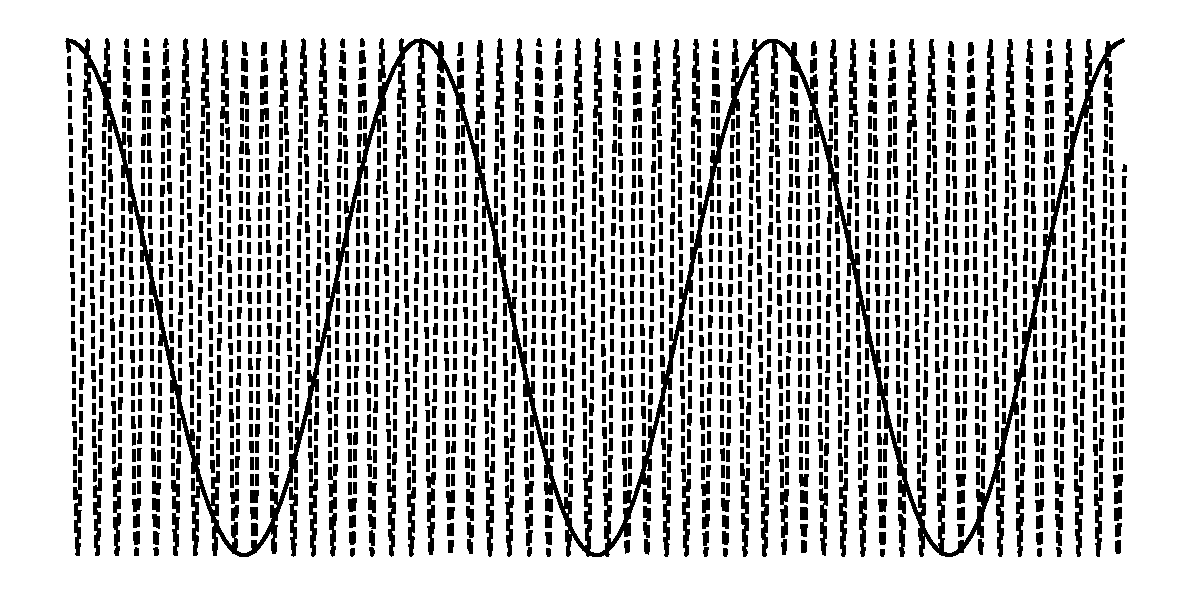
\includegraphics[width=\textwidth]
{figures/a440.pdf}}
\caption{\label{fig:my-label} A440 v. The Highest Note on a Piano}
\end{figure}

\subsection{The Quality of Sound - Superposition}
Now while pitch can certainly explain how we can tell the bass and the vocalist apart, how about sounds that are in the same range of pitch? For example a piano and our vocalist can both end up in in the same range of pitches and yet you'll still be able to tell them apart. What's going on here? Well, so far we've been oversimplifying things a lot. Remember how I said our picture of wave was the simplest picture possible? Well one of the ways in which it's super simple is that it's only got a single wavelength in it. In other words it has a single tone. Most sounds are not like this and are instead the composition of many wavelengths. This layering of wavelengths is called \textit{superposition} and it's best illustrated by an example. 

All sounds "begin" with a fundamental frequency - the lowest pitch in the sound. So let's begin with our simplest wave as the fundamental frequency (Fig 4.).

\begin{figure}[!htb]
\center{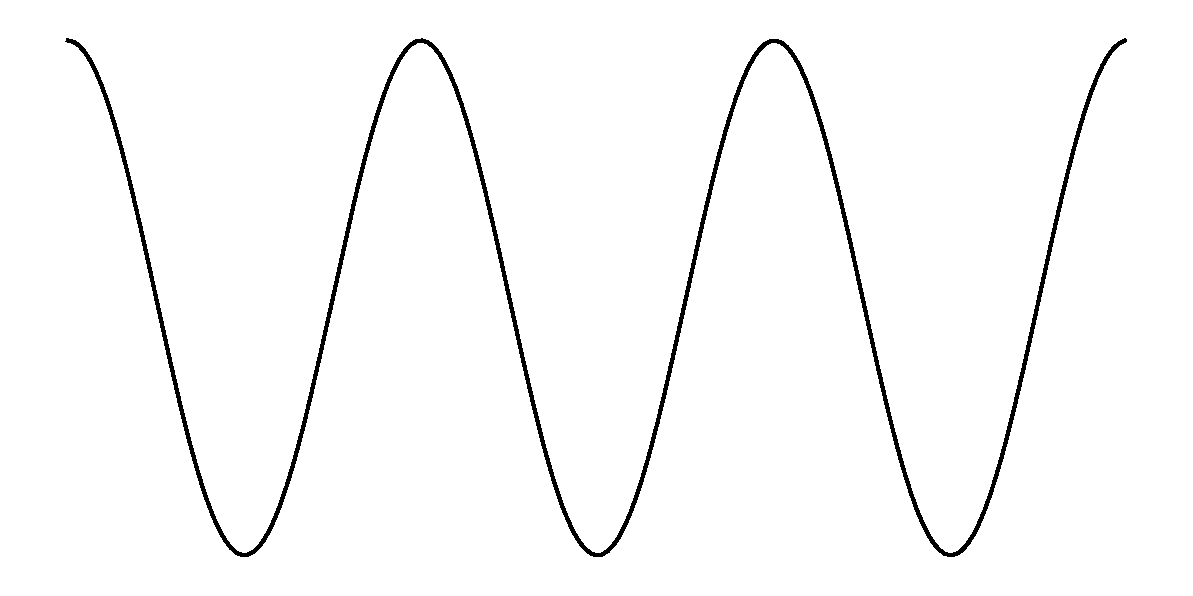
\includegraphics[width=\textwidth]
{figures/super1.pdf}}
\caption{\label{fig:my-label} Fundamental Frequency}
\end{figure}

With our fundamental frequency in place, let's add in our first higher frequency. Note that when superimposing waves, not only can their frequencies be different, but their amplitudes can be different as well (and almost always are). So to illustrate this we'll superimpose a wave with half the wavelength and half the amplitude on top of our fundamental frequency. Figure 5 shows both the two base waves (dashed) and the resulting superimposed wave (solid).

\begin{figure}[!htb]
\center{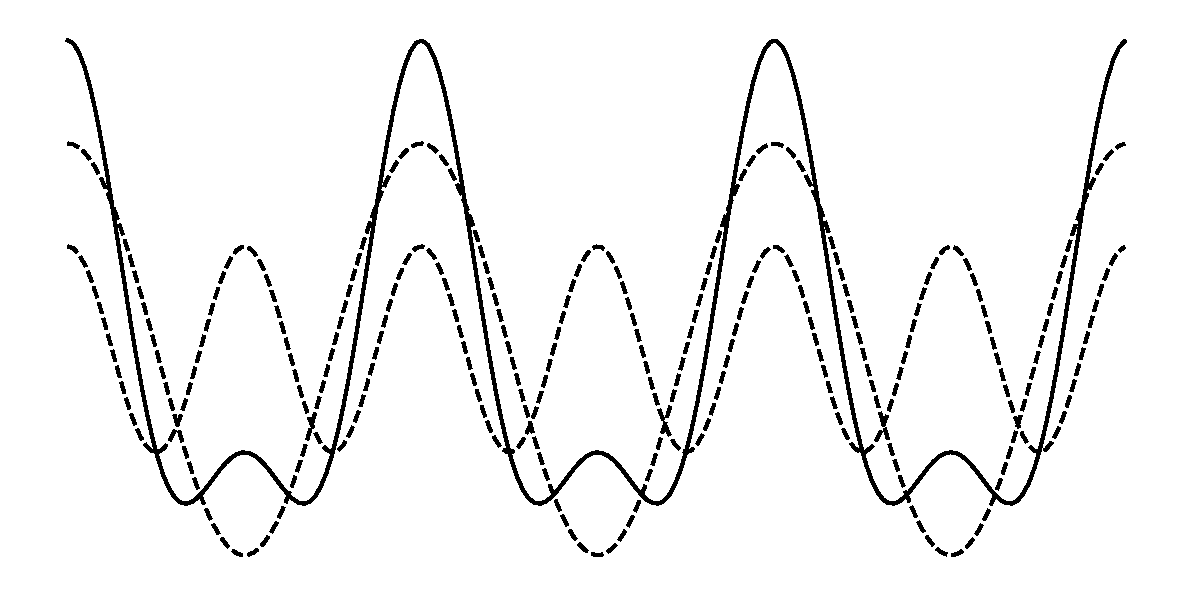
\includegraphics[width=\textwidth]
{figures/super2.pdf}}
\caption{\label{fig:my-label} Super Imposing Two Waves}
\end{figure}

Pretty wild right? (I find these kinds of waves starting looking really interesting and honestly kind of beautiful) 

Alright, let's add one more frequency in, this time with one quarter the wavelength and equal amplitude in comparison to our fundamental frequency (Fig. 6). 

\begin{figure}[!htb]
\center{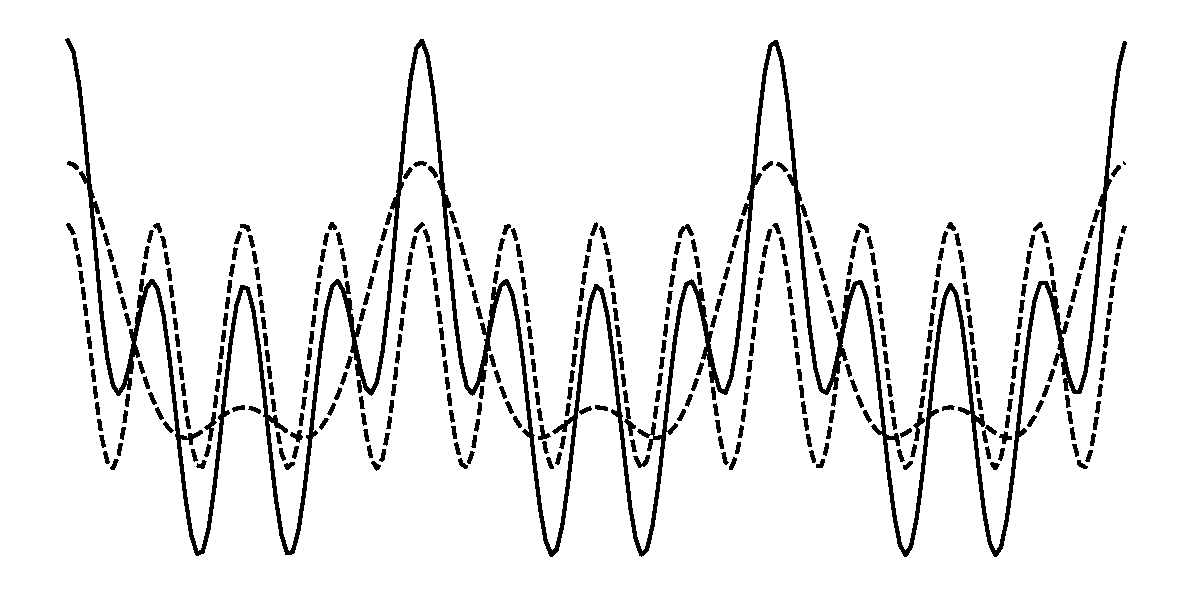
\includegraphics[width=\textwidth]
{figures/super3.pdf}}
\caption{\label{fig:my-label} Three Frequencies}
\end{figure}

Alright, while this is cool and nerdy and all, how does this relate back to distinguishing a piano from a vocalist? Well, when you play a note on any instrument the resulting sound is the superposition of whole load of different frequencies grounded on top of that fundamental frequency. What makes each instrument sound different, even when they're playing similar notes, is the fact that their particular mix of frequencies and amplitudes are each different. The combination particular to one instrument is what gives it its particular sound. In fact, for a trained ear, these differences can even allow you to identify one instrument from another. For example a piano with higher amplitudes at higher frequencies literally sounds brighter than one with muted amplitudes at higher frequencies. Superposition then, and the particular mix of frequencies and amplitudes that make up a specific sound, is yet another tool in our tool box of ways to distinguish one sound source from another. 

\subsection{Vanishing Act - Phase}
So we've now got amplitude, wavelength, and superposition which brings us to the final component we can use in describing our waves. This one is probably the most abstract and weird of the bunch, but it's one we're going to take advantage of a \textit{lot} and its name is \textbf{phase}. 

Thus far we've been looking at all of these waves as being in one spot in our graph. But there's no reason why we can't start shifting them from left to right (Fig 7.). This shifting is phase.

\begin{figure}[!htb]
\center{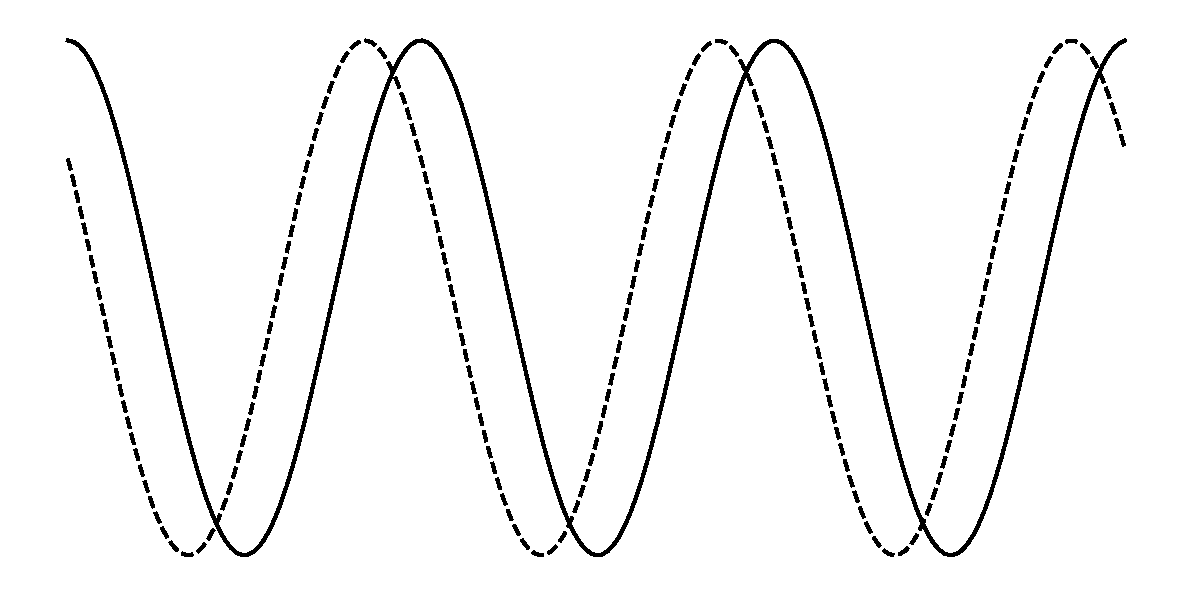
\includegraphics[width=\textwidth]
{figures/phase.pdf}}
\caption{\label{fig:my-label} Two Waves with Different Phases}
\end{figure}

What gets really weird (and where we start to see the power of phase) is when we superimpose two waves with the same wavelength but different phases. 

Figure 8 shows the super position of the two waves from Figure 7. Note how because the waves are nearly in sync (peaks match with peaks and troughs match with troughs) they add together to create a wave with much higher amplitude. This is known as \textbf{constructive interference}.

\begin{figure}[!htb]
\center{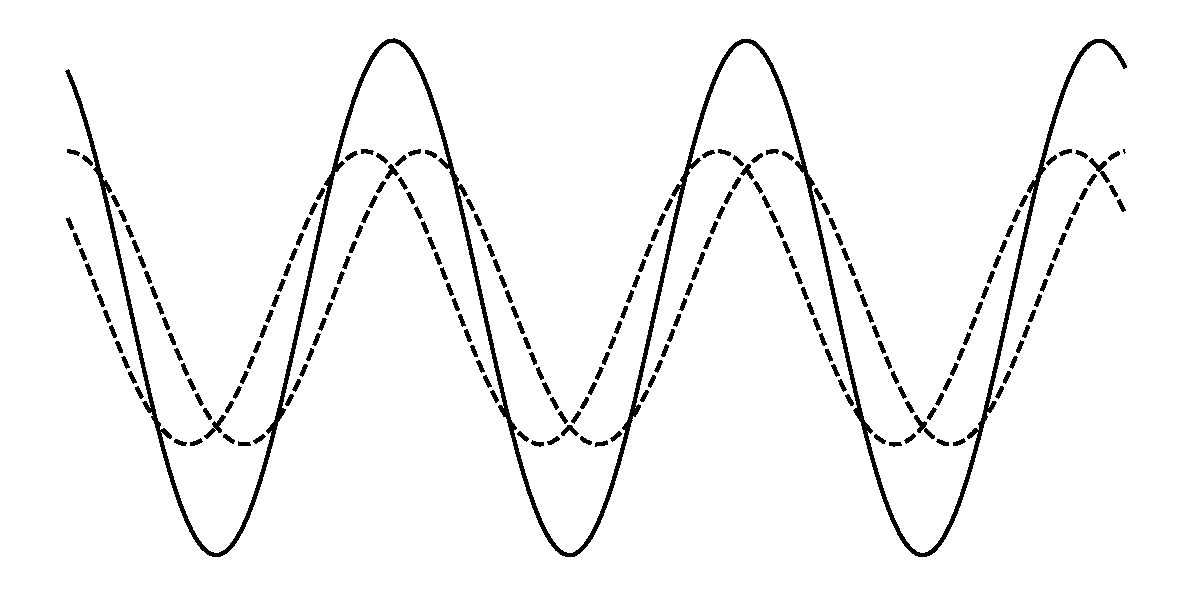
\includegraphics[width=\textwidth]
{figures/phasesuper1.pdf}}
\caption{\label{fig:my-label} Constructive Interference}
\end{figure}

On the other hand, Figure 9 shows the superposition of two waves that are nearly out of sync (peaks at troughs and troughs at peaks). Note how in this case the resulting wave is much smaller than either of the constituents - this is \textbf{destructive interference}.

\begin{figure}[!htb]
\center{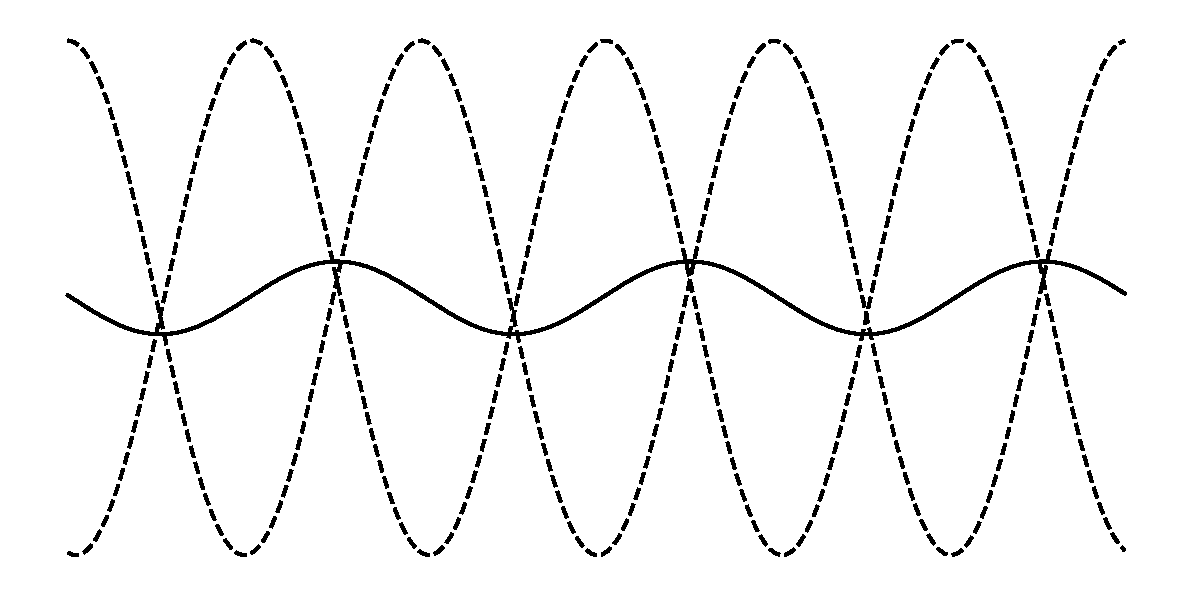
\includegraphics[width=\textwidth]
{figures/phasesuper2.pdf}}
\caption{\label{fig:my-label} Destructive Interference}
\end{figure}


What's really weird is that if you get the two waves to be exactly out of sync, the resulting superposition \textit{vanishes}! What does this mean physically? It means that the sound itself disappears! Yep, that's right, if two sound sources have just the right phase difference you'll suddenly no longer hear them even though the underlying sounds are there. Absolutely wild right? Well it turns out that this odd mathematical feature helps your brain figure out where sound is coming from.

Suppose a sound is coming directly from your right. That sound will obviously hit your right ear first. A very very short time later the same wave will hit your left ear, but at that point the undulation at your right ear will have changed (because the wave is constantly, well, waving). This difference in what your right and left ear are receiving is equivalent to the phase shift we were just talking about. Now suppose the sound is coming from directly in front of you. In this case the sound hits both ears at the same time because the distance to each ear is the same. This means there is no phase difference. What these two examples show is that as a sound source moves around your head the phase difference between your two ears changes. And your brain can use these differences to help you pick out where the sound is coming from! \cite{wikilocalization}. Pretty amazing, right? This happens to be the simplest version of a very cool technology called a \textbf{phased array} - something we'll be diving into detail next. But before we get to that we need to pull together all the tools we've gathered up so far and formalize them mathematically because phased arrays get pretty technical. So let's step back and do just that.

\subsection{Sums and Summaries - Mathematical Formalization}
Alright, so we've got all our pieces:
\begin{itemize}
\item \textbf{Amplitude:} The height of a wave, representing volume.
\item \textbf{Wavelength (or Frequency):} The width of a wave, representing pitch.
\item \textbf{Superposition:} The particular mix of amplitudes and frequencies that make up a sound.
\item \textbf{Phase:} An abstract sense of the "position" of a wave that leads to destructive or constructive interference.
\end{itemize}

How do we tie them all together mathematically? Well our simplest of waves is described by the following formula:
\begin{equation}
y=a e^{i\psi}e^{ikx}
\end{equation}
$e=2.71828$ is a mathematical constant known as Euler's number. $i=\sqrt{-1}$ is the imaginary number. $a$ is our amplitude. $k=2\pi/w$ where $w$ is our wavelength. Last but certainly not least, $\psi$ (pronounced like \textit{sigh}) is our phase. 

That then gets us three out of our four. So what about superposition? Well remember superposition is just adding many simple waves together, so we can do just that: 
\begin{equation}
y = a_1 e^{i\psi_1}e^{ik_1x} + a_2 e^{i\psi_2}e^{ik_2x} + ... + a_N e^{i\psi_N}e^{ik_Nx}
\end{equation}
Now writing out all these terms all of the time is going to get really burdensome, so we're going to take advantage of a little bit of mathematical notation that you may or may not be familiar with - the sum $\Sigma$. 

If you're not familiar with this notation, let's demonstrate with a simpler example. Suppose that you were adding the numbers 1 through 100. Without $\Sigma$ you would write:
\begin{equation}
1 + 2 + 3 + ... + 100
\end{equation}
With $\Sigma$ this same expression becomes:
\begin{equation}
\sum_{n=1}^{100}n
\end{equation}
which reads as - "add together all the $n$ (the thing to the right of the $\Sigma$) where $n$ starts at 1 (expression below the $\Sigma$) and goes all the way to 100 (number above the $\Sigma$)". I appreciate that this is probably pretty abstract and a little mind bending if this is your first time seeing it, but as we dive further into our little adventure you'll see just how useful this one bit of notation is. Alright, back to our waves.

Our superposition of waves goes from looking like this
\begin{equation}
y = a_1 e^{i\psi_1}e^{ik_1x} + a_2 e^{i\psi_2}e^{ik_2x} + ... + a_N e^{i\psi_N}e^{ik_Nx}
\end{equation}
to this:
\begin{equation}
y = \sum_{n=1}^{N}a_n e^{i\psi_n}e^{ik_nx}
\end{equation}
which is far neater and, as will become clear later, far easier to work with. 

That's it then! We've got our equation for a wave and are clear on the various components that make one sound different from another. With these tools in hand let's go and look at an absolutely incredible (and mathematically beautiful) technology for sound localization based on nothing more than our two ears - the phased array. 

\newpage
\section{To Phase Array}
\subsection{Back at the Pond}
With a firmer understanding of the components of sound, let's return to the pond.  Frogs in full chorus are a tricky bunch because while different species of frog may sound quite different, the individuals within a species are much more like instruments in the same section - while we find it easy to distinguish the violins from the cellos, telling individual cellos apart is extremely difficult (unless someone is playing terribly off tune). This is because they've all got roughly the same pitch, are playing at nearly the same time, and have similar if not identical volumes. Frogs, surprisingly are quite the same. The song for a specific species is very distinct, in chorus they tend to overlap with one another, and, in the competition to be heard, everyone gets rather loud. To complicate things even further they'll vary the length or repeats in their songs so we can't even try to identify a specific phrase as an individual. So, if frequency and amplitude are so unhelpful to us at this specific stage what are we to do? 

What we do know is that each frog is going to be calling from a specific spot - so while they may overlap in terms of a lot of things, position is unlikely to be one of them. This brings us straight back to our two ears example from the last section. Recall how as you vary the position of what you're listening to, the difference in timing between your two ears changes and that these differences in timing correspond to differences in phase. Well this means that if you have multiple listening devices (in this case your two ears), the phase differences between those sources is a function of the position of the sound source. How does this help us? Well remember that phase differences create destructive and constructive interference; so, if the phase difference is a function of location so too is whether the interference is constructive or destructive. 

Let's take an example (and note this is an illustrative example, the extent to which your brain actually does this is up for debate). Suppose that we have two sound sources. One directly in front of you and one directly to the right. For the source directly in front of you, the distance from the source to each of your ears will be exactly the same. Therefore, the phase difference will be zero and as we saw in Section 2.4 this will mean perfect constructive interference - the combined wave will have twice the amplitude. Now consider the sound source at your right. Obviously the sound from that source will hit your right ear first and then your left. Suppose that the wavelength of this wave is such that when the sound hits your left ear it is at a peak but when it hits your right ear it is at a trough - i.e. they are completely out of sync. In this case we'll get perfect destructive interference and the superimposed sound will vanish. Now note this doesn't mean you'll just stop hearing the sound because your brain can do all sorts of funky things with the sounds coming to your ears; but, if we imagined two microphones reading in these sounds and superimposing them it would hear the sound in front as twice as loud and the sound to the right not at all which means we'd have a way of listening to one location while completely ignoring another which is exactly what we want!

Let's take this a step further. Returning to our digital ears (the microphones) we know that we can post-process the data from each microphone however we like. In other words, we can delay the signals coming from either microphone before combining them. So for example, we could delay the signal at the right microphone so that we get the two signals from the right sound source to line up and experience constructive interference. But this will of course cause the sound source at the front to go out of phase and vanish. In other words, using digital post processing we've switched which location we're listening too! And because it's digital, we can do both the delay and no delay at the same time as two separate processes which means we can isolate each sound source and listen to them simultaneously!

Now imagine that we had a setup like this at the pond. In theory it may be possible for us to vary the delays on our digital ears in such a way that we could isolate many different locations on the pond surface simultaneously and listen to them all at once. If we can get the size of those isolated blocks to be small enough that they cover a single frogs territory then we could listen to all the frogs individually and have broken the frog cipher! 

Well turns out this kind of setup is an already well developed technology known as a \textbf{phased array}. But phased arrays require a great deal of precision and far more than two digital ears. So in order to figure out how this would work in reality we're going to need to go through the mathematics of phased array antennas - the subject of the rest of this section. Then in the following section we'll be able to return to the question of what it would take to build a phased array antenna that could listen to individual frogs on a pond simultaneously. So let's dive into the math. 

\subsection{On Many Eared Aliens - Planar Phased Arrays}
The following derivations and treatment come almost entirely from an absolutely incredible book - \textit{Phased Array Antenna Handbook} \cite{phasedhandbook}. If you're wanting to go into more detail or learn more about phased array antennas I'd encourage you to check it out. 

We begin with a large grid sitting, as all things mathematical tend to do, on a plane (a big, perfectly flat surface). This grid is composed of lovely, omni-directional antennas. Specifically they are layered $M$ deep with a spacing of $d_x$ along the $x$-axis  and $N$ deep with a spacing of $d_y$ along the $y$-axis which means we have $M\times N$ antennas in total. This setup is known as a planar phased array antenna. We denote the position of our sound source by two angles (illustrated in Figure 10) $\theta$ and $\phi$. 

\begin{figure}[!htb]
\center{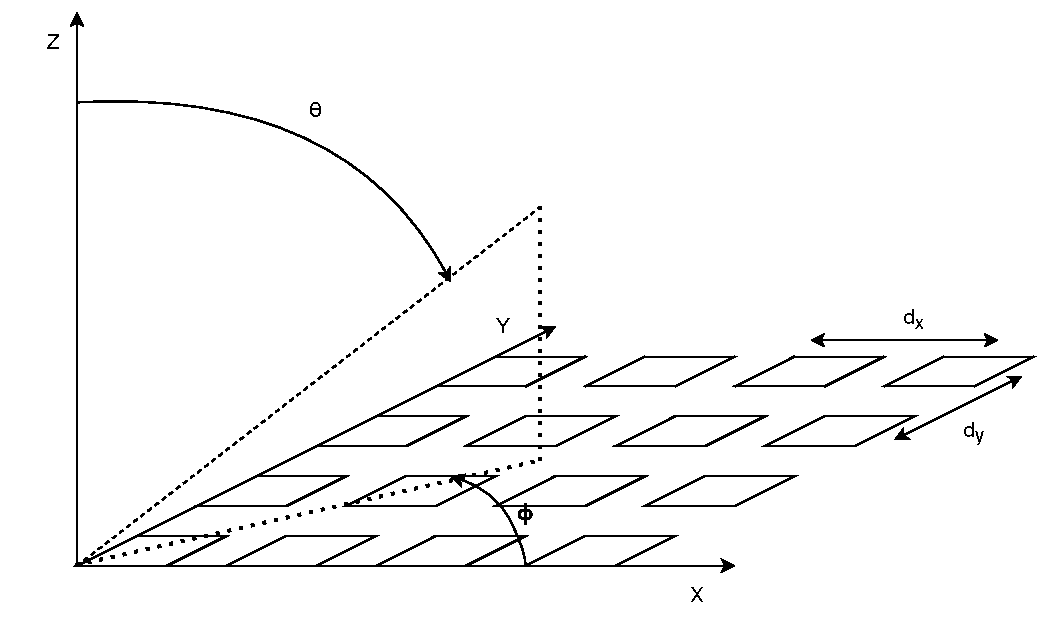
\includegraphics[width=\textwidth]
{figures/phased_array_diagram.pdf}}
\caption{\label{fig:my-label} A Planar Phased Array}
\end{figure}


You'll remember from the prior section that our overall wave equation for a single frequency was given by:

\begin{equation}
y = a e^{i\psi}e^{ikx}
\end{equation}

Our independent variable here was $x$ which in that context was the distance from the sound source to the position you were observing the wave at. Given we're using $x$ for something else in this context (one of the dimensions of our planar phased array) we'll instead designate the distance from our sound source to the $j$th element of our array as $R_j$. In other words:


\begin{equation}
y = a e^{ikR_j}
\end{equation}

Note that we're ignoring the phase term here because for a single wave it's just a constant and will therefore have nothing to do with our constructive or destructive interference. 

Now it's important to note that we're making a  few simplifications here. First, in reality as you get farther from a sound source the amplitude shrinks but we're just assuming we're only interested in the amplitude near the antenna $a$ so we don't need to account for this reduction in sound level. Second we're implicitly making what's called a \textit{far field} assumption here - namely that the source is far enough away that we can use our simple wave equation from the last section (if the sound source is very close the equation gets far more complicated). We'll get into what this means for our antenna design in the next section, but I figured it would be useful to mention now. 

Let's next go ahead and designate $R$ to be the distance from the sound source to our our origin $(0,0)$, $\mathbf{\hat{r}}$ as the unit vector from the origin in the direction of our sound source, and $\mathbf{r_j}$ as the vector from the origin to the $j$th element (see Figure 11). In the case where $R_j$ is very large we find:

\begin{equation}
R_j \approx R - \mathbf{\hat{r}}\bullet\mathbf{r_j}
\end{equation}

Why is this useful? Well let's look at what $\mathbf{\hat{r}}\bullet\mathbf{r_j}$ ends up being. Using Figure 10, some trigonometry, and the definition of our planar array we find that:

\begin{equation}
\mathbf{r_j} = \mathbf{\hat{x}}x_j + \mathbf{\hat{y}}y_j + \mathbf{\hat{z}}z_j
\end{equation}

\begin{equation}
\mathbf{\hat{r}} = \mathbf{\hat{x}}\sin \theta \cos \phi + \mathbf{\hat{y}}\sin \theta \sin \phi + \mathbf{\hat{z}}\cos \theta
\end{equation}

where $\mathbf{\hat{x}}$, $\mathbf{\hat{y}}$, and $\mathbf{\hat{z}}$ are our coordinate vectors and $x_j,y_j,z_j$ are the coordinates of our $j$th antenna. Let's define $u=\sin \theta \cos \phi$ and $v=\sin \theta \sin \phi$ so that we can shorten the latter equation to:

\begin{equation}
\mathbf{\hat{r}} = \mathbf{\hat{x}}u + \mathbf{\hat{y}}v + \mathbf{\hat{z}}\cos \theta
\end{equation}

Next if we define $m$ to be the number of antennas in our $j$th antenna is along the $x$-axis and $n$ the same along the $y$-axis then we have:

\begin{equation}
 \mathbf{\hat{x}}x_j + \mathbf{\hat{y}}y_j + \mathbf{\hat{z}}z_j =  \mathbf{\hat{x}}md_x + \mathbf{\hat{y}}nd_y
\end{equation}

So now we can go ahead and compute the scalar product:

\begin{equation}
\mathbf{\hat{r}}\bullet\mathbf{r_j}=qd_xu+pd_yv
\end{equation}

Plugging this into our approximation we have:

\begin{equation}
R_j \approx R - qd_xu+pd_yv
\end{equation}

Still unsure what all this juggling has been for? Well let's throw this back into our wave equation and see what this is all about:

\begin{equation}
a e^{ikR_J} \approx a e^{ik(R - qd_xu+pd_yv} = ae^{ikR}e^{-ik(qd_xu+pd_yv)}
\end{equation}

Note that $e^{ikR}$ is once again just a constant phase term that we don't care about here and that because we're interested in the value of the phase and not its sign we don't care about the negative in front of $ik(qd_xu+pd_yv)$ either. Therefore this all simplifies to:

\begin{equation}
ae^{ik(qd_xu+pd_yv)}
\end{equation}

Which means our whole wave equation is now defined entirely in terms of values we know - pretty slick. 

\begin{figure}[!htb]
\center{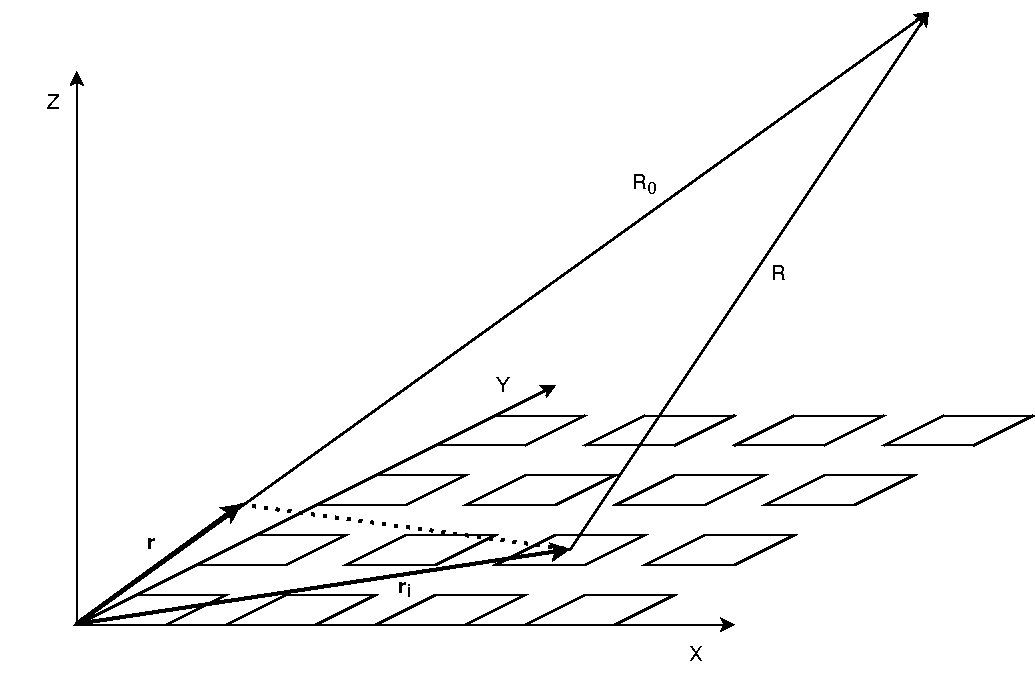
\includegraphics[width=\textwidth]
{figures/R_approx.pdf}}
\caption{\label{fig:my-label} Approximation of $R_j$}
\end{figure}

Alright, thus far we've only been talking about what the microphone sees without modifications. But remember that the whole point here is going to be introducing phase shifts in order to create the constructive or destructive interference that we want. A phase shift is simply represented by adding (or subtracting) a value from our exponent:

\begin{equation}
ae^{ik(md_xu+nd_yv)}e^{i\psi}
\end{equation}

Now if we set $\psi$ so that it cancels the other exponent we'll find that all antennas (regardless of the specific $m$ or $n$) will have the same phase. I.e. we will be creating the maximal constructive interference for the direction defined by $\theta$ and $\phi$. Therefore:

\begin{equation}
\psi=-k(md_xu+nd_yv)
\end{equation}

Let's generalize this a little bit. Let's create two new variables $u_0=\sin \theta_0 \cos \phi_0$ and $v_0=\sin \theta_0 \sin \phi_0$ that designate our \textbf{steering angle}. Then let's set $\psi=-k(md_xu_0+nd_yv_0)$ so that our wave becomes

\begin{equation}
ae^{ik(md_x(u-u_0)+nd_y(v-v_0))}
\end{equation}

From here it becomes clear that when the steering angle and the source direction coincide we get the most constructive interference (because all of the antennas experience the same phase regardless of $m$ and $n$).

You may now be wondering what happens when the steering angle and the source direction don't coincide. Well the contributions from all of our $M\times N$ antennas is:

\begin{equation}
I=\sum_{m=1}^M \sum_{n=1}^N  ae^{ikqd_x(u-u_0)}e^{ikpd_y(v-v_0)}
\end{equation}

so let's plot out some examples and see! (Also imagine trying to write out that equation without our $\Sigma$ notation...)

\subsection{Enough Math, Show Me Something}
We've got a mathematical formalization for our phased array so it's time to check out what things actually look like! Let's take a simple example of a single row of antennas (i.e. $N=1$) and graph things out!

Now for those of you who have been playing close attention you'll have noticed that the $I$ from the preceding subsection is an imaginary number. Obviously we won't be plotting anything imaginary so what are we going to be plotting? We'll be plotting the power as a function of $\theta$ (the source location). Power is defined as:

\begin{equation}
P=I\bar{I}
\end{equation}

or as $I$ multiplied by it's conjugate. 

As a final note before we get plotting we're going to be plotting the power in $dB$ relative to the maximum power. That just means we're going to be using a log scale rather than a linear one. Alright let's get to it.

We'll start with the simplest case where $u_0$ (indicative of the \textbf{steering angle}) is steered to $\theta=0$ (Figure 12). We'll include 10 elements in our array and space them half a wavelength apart (more on this in the next section). 

\begin{figure}[!htb]
\center{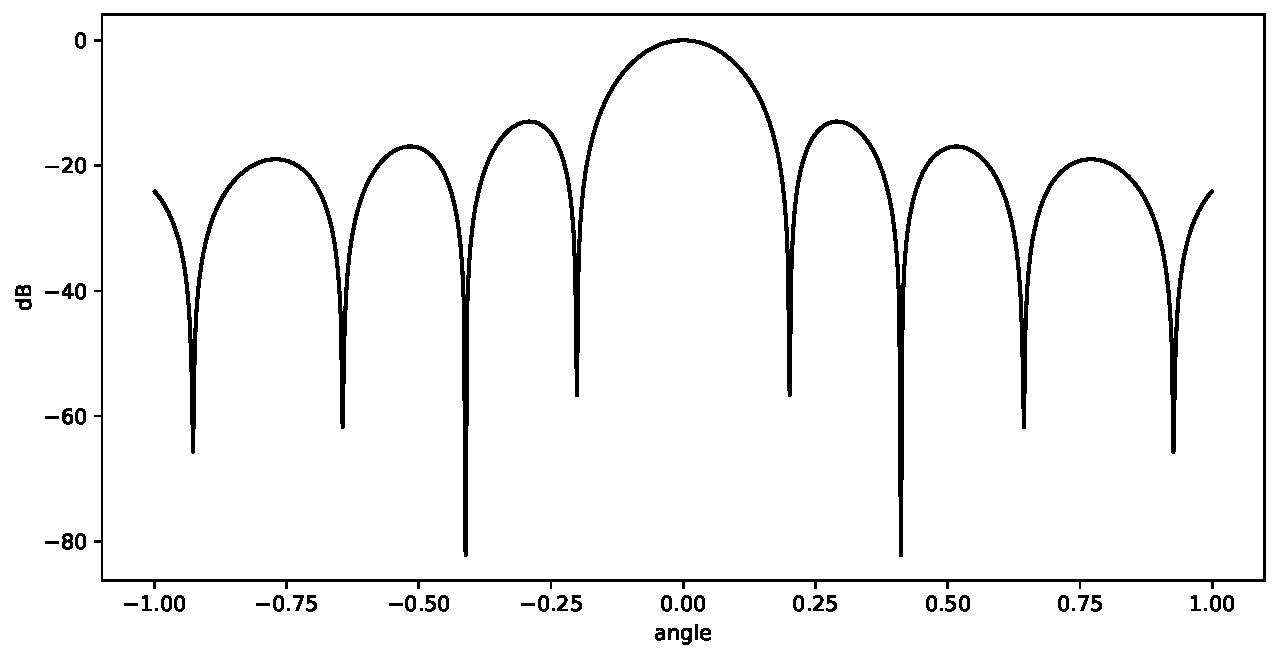
\includegraphics[width=\textwidth]
{figures/steer0_el10.pdf}}
\caption{\label{fig:my-label} Steering Angle $\theta=0$ with 10 Element Array}
\end{figure}

Right away there's several things to take away from this graph. First while we have steered toward $\theta=0$ and are getting our most constructive interference at that angle, it's not as if the constructive interference just falls off immediately as we move away from $\theta=0$. Instead we see that we have this whole area around $\theta=0$ where we still have considerable power before it drops off sharply. That area is known as the \textbf{beam} and its width (measured in various ways) is the \textbf{beam width}. Put another way, we won't just be hearing things at $\theta=0$ but also things throughout the beam. How narrow our beam is (and thus how small the beam width) determines how localized our listening will be. 

Second, in the graph we see these steep drop offs followed by subsequent peaks. These other peaks are known as \textbf{sidelobes} and are other areas in which we'll get non-negligible signal from. 

Let's now look at a couple other examples. First let's see the effect of changing the steering angle by modifying our $u_0$ (Figure 13). 

\begin{figure}[!htb]
\center{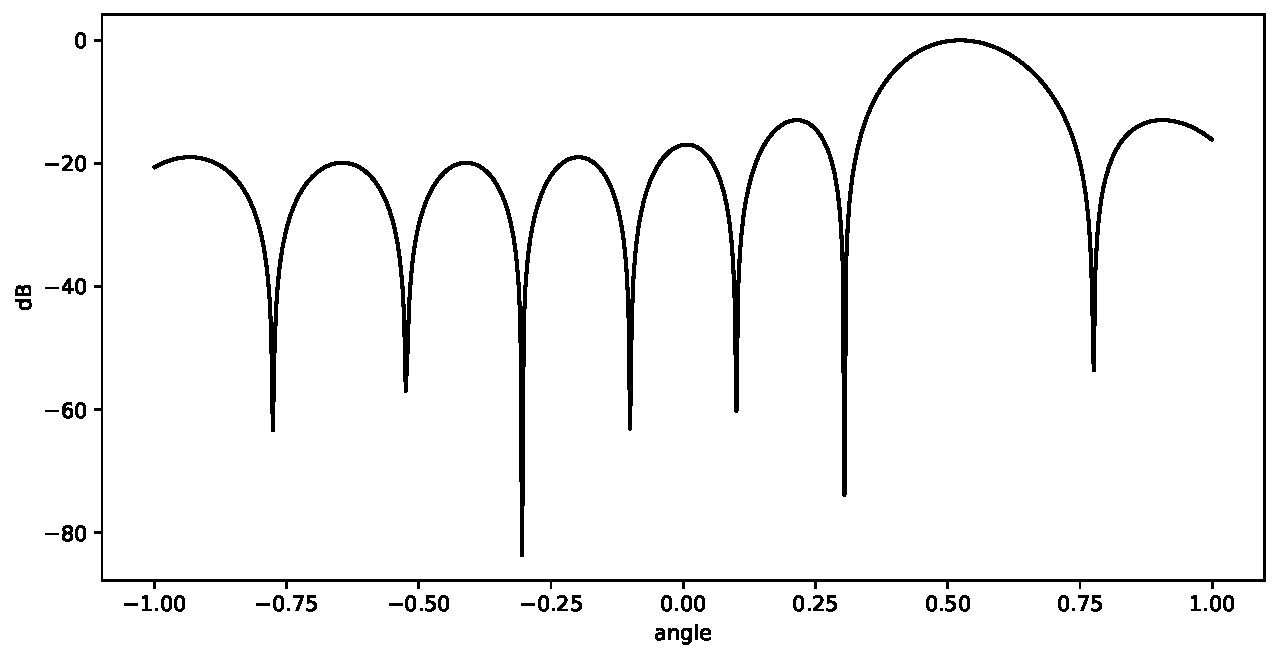
\includegraphics[width=\textwidth]
{figures/steerpi6_el10.pdf}}
\caption{\label{fig:my-label} Steering Angle $\theta=\pi/6$ with 10 Element Array}
\end{figure}

This is exactly as we'd expect, as the steering angle changes the position of our beam should change as well. 

Finally let's look at what happens when we increase the number of elements to 20 (Figure 14).

\begin{figure}[!htb]
\center{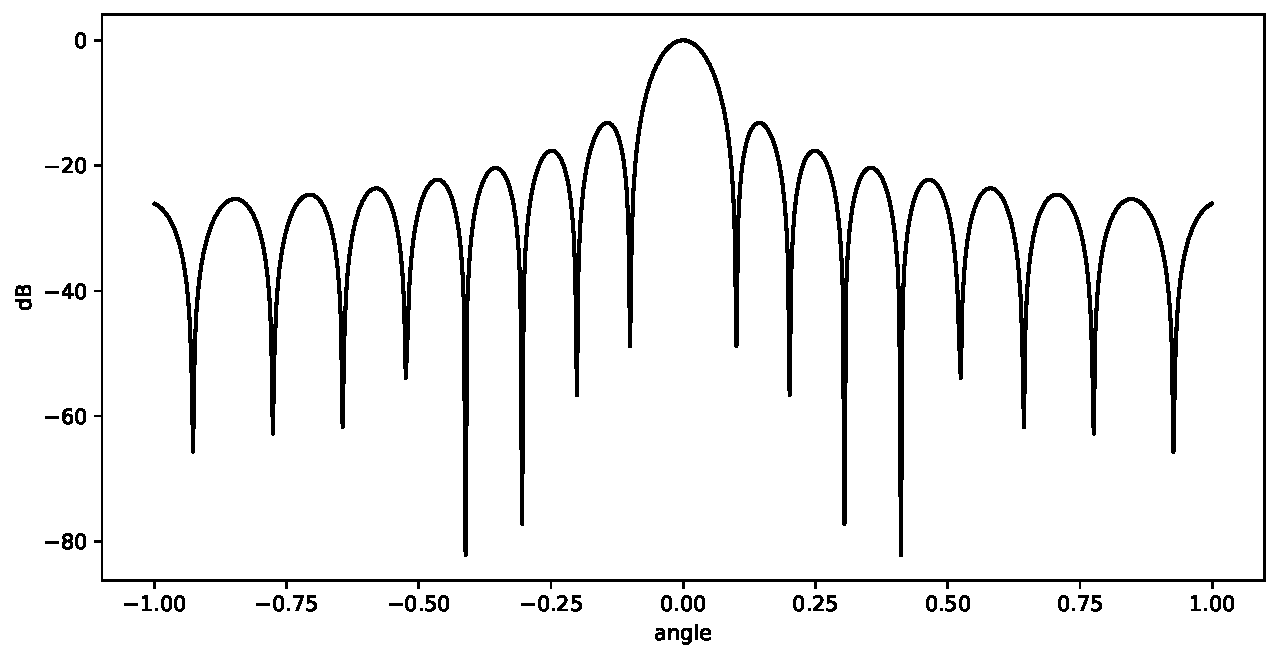
\includegraphics[width=\textwidth]
{figures/steer0_el20.pdf}}
\caption{\label{fig:my-label} Steering Angle $\theta=0$ with 20 Element Array}
\end{figure}

Notice how in comparison to our 10 element array our beam width has shrunk dramatically. In general, as we add elements our localization improves and where we receive signal from shrinks. This is our first aspect of antenna design - a subject we'll now turn to in more detail in order to understand what it would take to localize all the frogs on the surface of a pond. 

\newpage


\section{How Tall is A-flat?}
We have formalized our phased array with the following equation:

\begin{equation}
I=\sum_{m=1}^M \sum_{n=1}^N  ae^{ikqd_x(u-u_0)}e^{ikpd_y(v-v_0)}
\end{equation}

Which shows us pretty summarily that the two things we have control over are (1) the number of elements ($M$ and $N$) and (2) the spacing of those elements ($d_x$ and $d_y$). So let's understand how changing each of these changes the properties of our phased array antenna. 

\subsection{Getting Greedy - Number of Elements}
The first of our modifiable parameters is the number of elements. We already saw the main gist of what happens here when we went from 10 to 20 elements in the last section and saw the beam width shrink. But, to firm up our intuition and understanding, let's go through a few more examples. 

We'll iterate from the simplest array possible at 2 elements through 4, 16, and then 256 elements (Figures 15 - 18). 

\begin{figure}[!htb]
\center{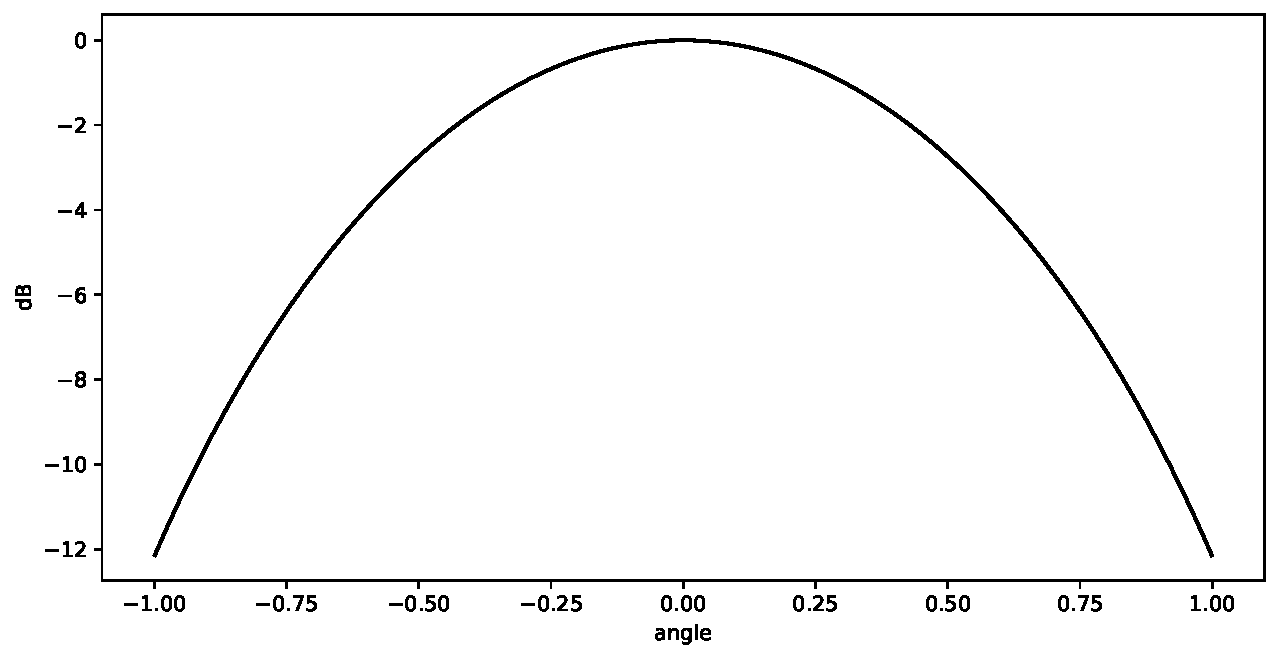
\includegraphics[width=\textwidth]
{figures/2elements.pdf}}
\caption{\label{fig:my-label} Steering Angle $\theta=0$ with 2 Element Array}
\end{figure}

\begin{figure}[!htb]
\center{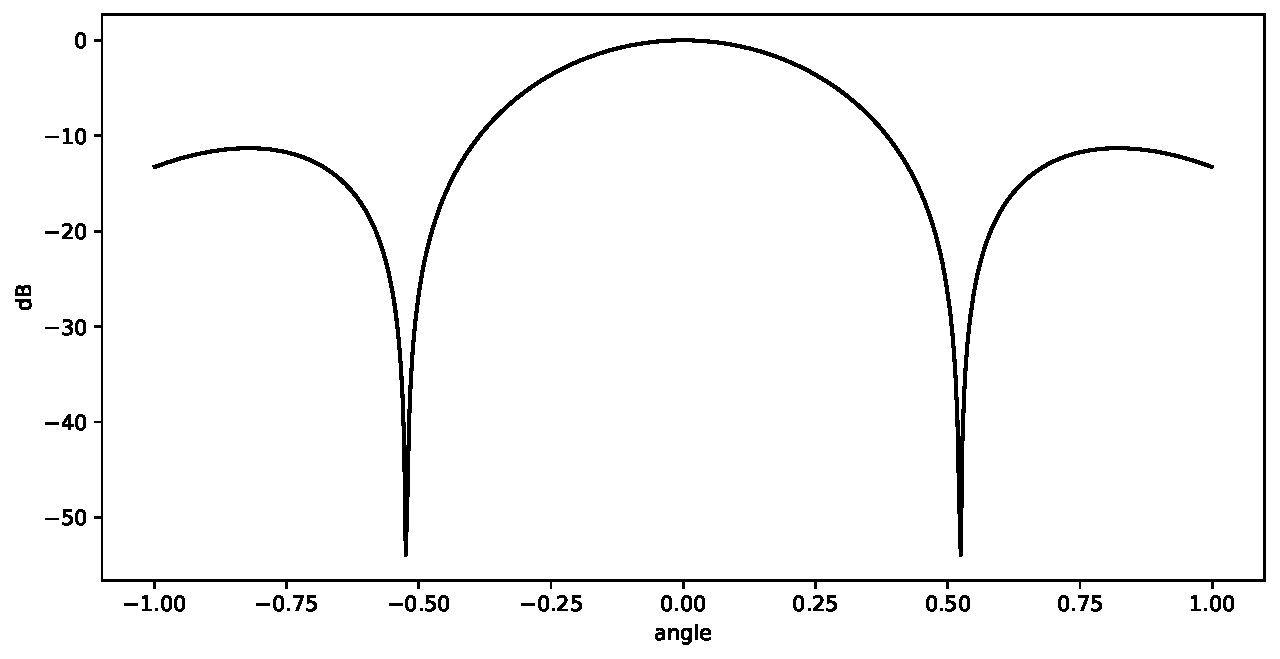
\includegraphics[width=\textwidth]
{figures/4elements.pdf}}
\caption{\label{fig:my-label} Steering Angle $\theta=0$ with 4 Element Array}
\end{figure}

\begin{figure}[!htb]
\center{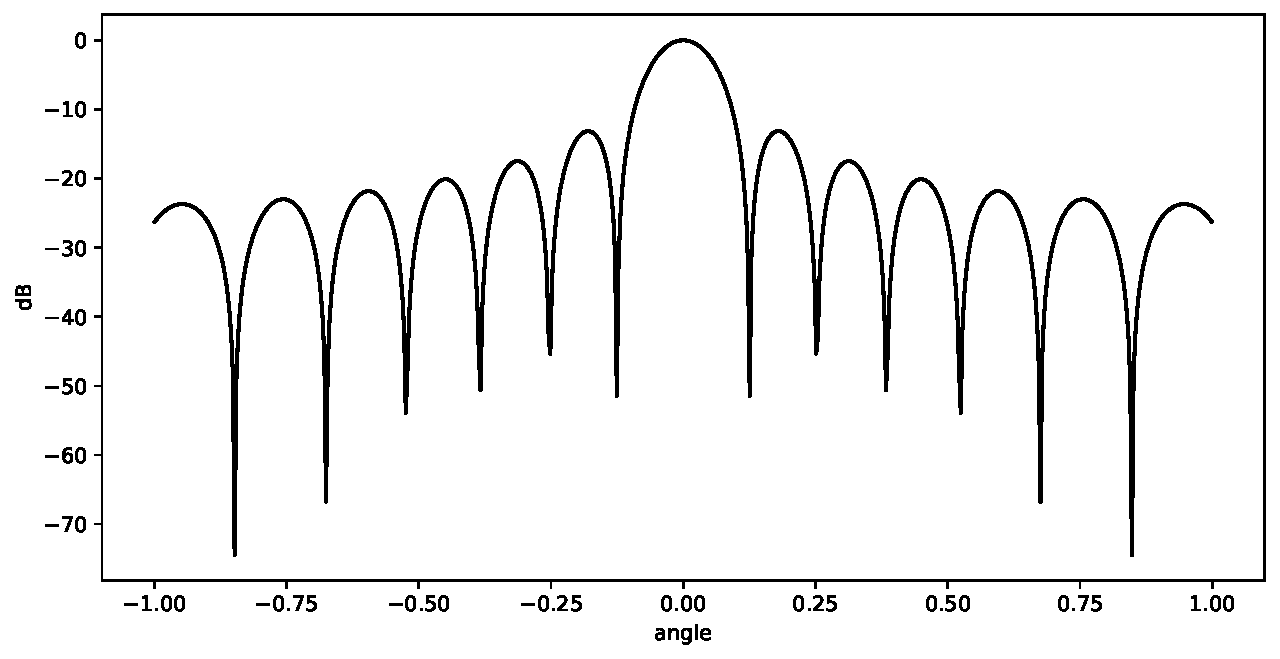
\includegraphics[width=\textwidth]
{figures/16elements.pdf}}
\caption{\label{fig:my-label} Steering Angle $\theta=0$ with 16 Element Array}
\end{figure}

\begin{figure}[!htb]
\center{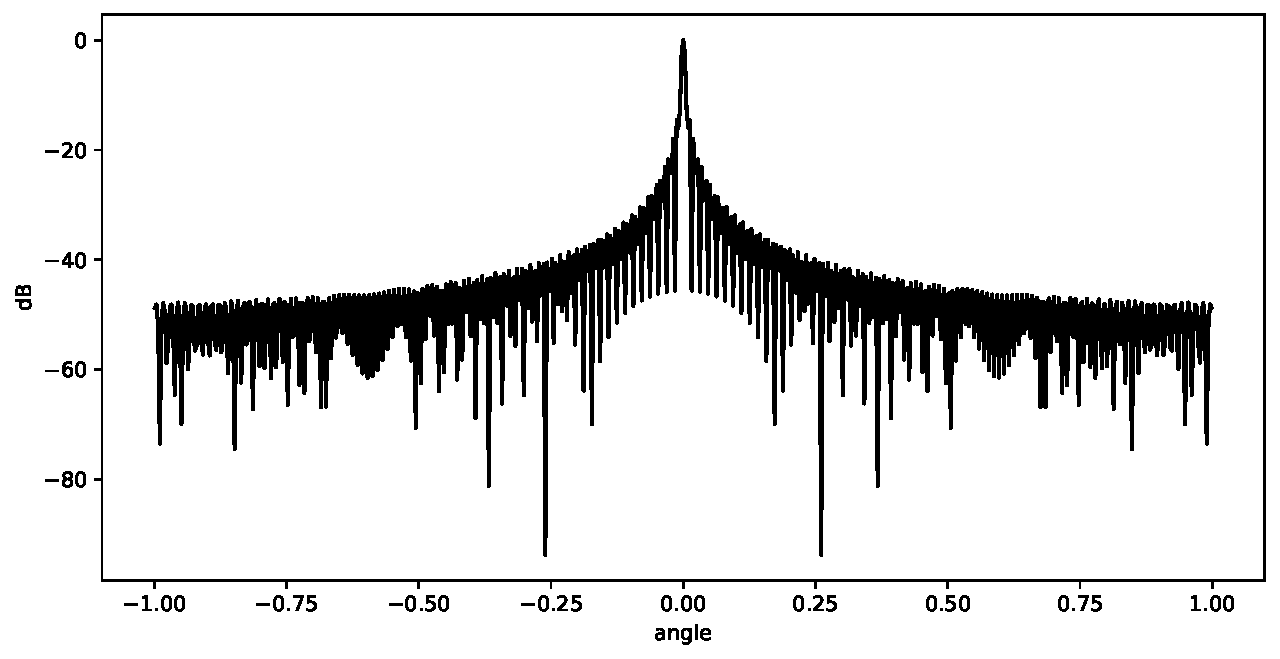
\includegraphics[width=\textwidth]
{figures/256elements.pdf}}
\caption{\label{fig:my-label} Steering Angle $\theta=0$ with 256 Element Array}
\end{figure}

The first take away from this sequence is both how wide the beam is in the case of two elements and how we can make it more or less indefinitely small by adding more and more elements (look at how small the beam width is in the 256 element case!). The second point of note, though, is that as the beam width shrinks the number of distinct side lobes increases. While an interesting observation this is not going to be of huge concern to us. Main takeaway should be that if you want to shrink your beam width - add more elements. 

\subsection{Being Skinny Isn't Always Great - Element Spacing}
Next we have our good ole spacing parameters $d_x$ and $d_y$ (or just $d_x$ as we're considering a one dimensional phased array at the moment). Let's return to our 10 element phased array with what we called half wavelength spacing (Figure 19):

\begin{figure}[!htb]
\center{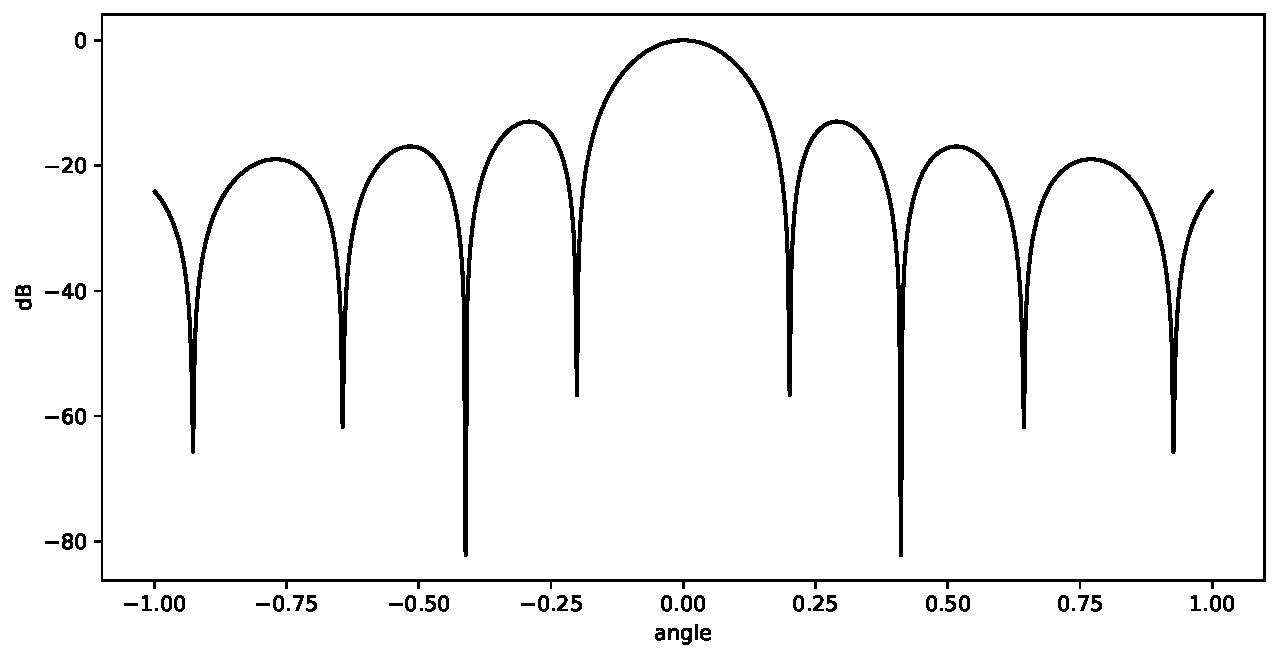
\includegraphics[width=\textwidth]
{figures/steer0_el10.pdf}}
\caption{\label{fig:my-label} Half Wavelength Spacing}
\end{figure}

First let's drop the spacing to, say, a quarter wavelength (Figure 20). Note our beam width just increased! This makes sense because as our elements get closer and closer they become more and more like one single antenna rather than a phased array. Does that then mean that the larger our spacing the better? Not quite. To illustrate why consider the case of two wavelength spacing (Figure 21). 

\begin{figure}[!htb]
\center{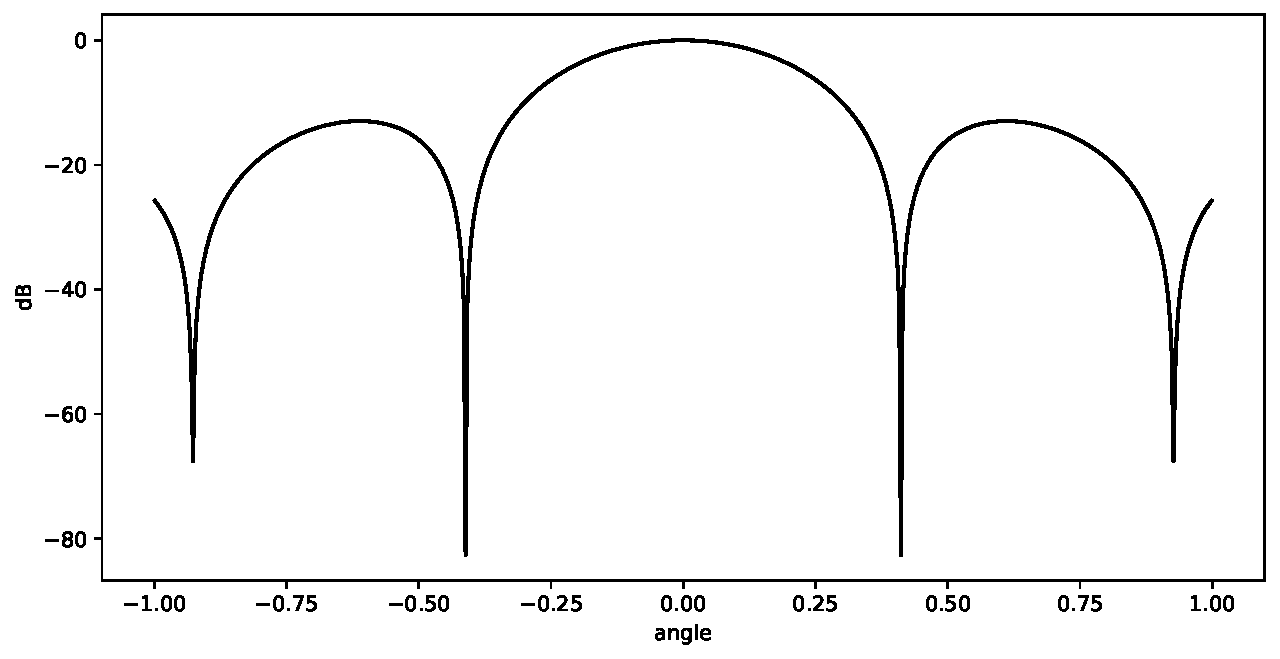
\includegraphics[width=\textwidth]
{figures/quarter_wavelength.pdf}}
\caption{\label{fig:my-label} Quarter Wavelength Spacing}
\end{figure}

\begin{figure}[!htb]
\center{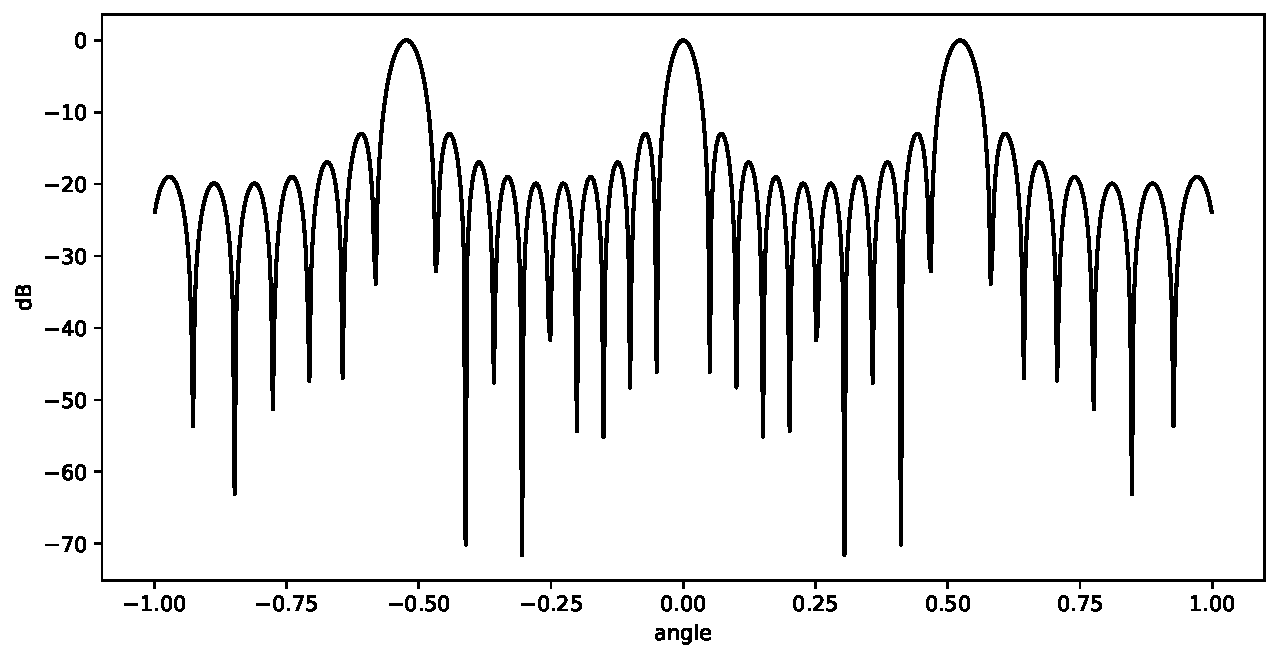
\includegraphics[width=\textwidth]
{figures/two_wavelengths.pdf}}
\caption{\label{fig:my-label} Two Wavelength Spacing}
\end{figure}

What the on earth is going on here?! We now see multiple beams! This comes down to a degeneracy in any kind of cyclic function. Remember how we were getting constructive interference because the phases were all the same across all the antenna elements? Well this is not the only way to get perfect constructive interference. Phases that are different by exact multiples of $2\pi$ will also create perfect constructive interference. Looking back at our equation for our phased array

\begin{equation}
I=\sum_{m=1}^M \sum_{n=1}^N  ae^{ikqd_x(u-u_0)}e^{ikpd_y(v-v_0)}
\end{equation}

we can see that as $d_x$ or $d_y$ increase, changes in the $u-u_0$ or $v-v_0$ have a larger overall impact on the phase of the exponential. Therefore as the spacing increases it becomes possible to hit multiples of $2\pi$ and thereby create other areas of perfect constructive interference (our other beams in the graph). These other beams are known as \textbf{grating lobes}. Note too that $k$ plays a similar role to $d_x$ and $d_y$ which is why spacing has to be a function of the wavelength. In general, the rule of thumb is that larger spacing is always better but to avoid grating lobes you need to keep the spacing $\leq$ to half the wavelength. 

\subsection{Far A Field}
Okay, we've talked about the number of elements and the spacing of elements. That's it right? Not exactly. Remember how I mentioned in the last section that we were making a far field assumption? Well it's time to talk about that now and what it means for the design of our antenna. 

In almost every case thus far we've been talking about planar waves - that is waves that look like they're coming in a single front. To get a sense of what I mean by this, a planar wave is kind of like what happens if you were to take a sheet and wiggle it. Each of the waves travels straight down the sheet without radiating in some new direction. Compare this on the other hand to what happens when you drop a stone in a pond. Those waves radiate outwards in all directions in rings. 

Close to a sound source waves are much more like what you see on the surface of a pond and, unsurprisingly, the math involved is a lot more complicated than what we've been going over here. But if you imagine that circular wave radiating out really really far and looking at only a small part of that circumference you'll note that as the radius of the circle gets larger, the edge gets flatter - in other words it becomes more and more like a planar wave. This is the far field assumption (or perhaps the better word would be simplification) - as you get far from the source of the wave the wave becomes approximately planar. 

How far away do you need to be for this to take effect? The answer is known as the \textbf{Fraunhofer distance} \cite{wikifarfield}:

\begin{equation}
\frac{2D^2}{w}
\end{equation}

where $w$ is the wavelength and $D$ is the largest dimension of the antenna. If we assume a half wavelength spacing between elements then for a linear array this becomes:

 
\begin{equation}
\frac{2(w/2(M-1))^2}{w}=\frac{w}{2}(M-1)^2
\end{equation}

In other words as either our wavelength or the number of elements we use increases, the far field gets farther and farther away. 

Okay so let's take everything we've learned and put it together to see whether simultaneous listening with a phased array antenna is even possible. 

\subsection{Sound is Big - Designing the Antenna}

As has probably become clear from the last few subsections, the two most important parameters for us are - what's the wavelength we're going to be listening in at and how tight does our beam need to be? 

Let's start with a rather well known critter - the Coqui (for which I've read several studies on automated call recognition). A reasonable middle for their frequency range is 2000 Hz \cite{mlcoqui}. Given the speed of sound is roughly 343 m/s this corresponds to a wavelength of $343/2000\approx 0.17$m (about 6.7 inches). Right off the bat then we know that we're spacing our antennas $3.3$inches apart. 

Next, what's the beam width we want? Let's suppose the frogs are, at a maximum, 10 meters away. Using some trigonometry we can derive that a beam width of 5 degrees ($\approx 0.09$ radians) would therefore correspond to $2\times 10 \tan(0.09/2)\approx0.9$m. This is probably too large so let's try a 2.5 degree beam which will give us about half a meter width at 10 meters distance. 

How many elements are required to get a 2.5 degree width? Well looking 3dB down from peak (half power down) and varying the number of elements in our linear array the answer is $\approx 45$. 45 elements to a side means $45\times45=2025$ distinct antennas! It also means an antenna that's $(45-1)*0.17\approx 7.5$m wide! Not only is this just far too wide to handle it also means our far field would only begin far past our 10m limit that we were talking about earlier. 

So what's going on here? Why have we come to the conclusion that we're going to need a house sized antenna? The answer is unfortunately quite simple. Sound waves are actually quite large and therefore don't allow us to provide very high resolution. It's like the difference between a light microscope and an electron microscope. An electron microscope can allow you to see individual atoms because the wavelengths used by the microscope are so much smaller (and therefore much higher resolution) than the ones used in a light microscope. Meanwhile we're over here trying to use wavelengths that are the size of a hand and larger! Clunky resolution indeed. 

So is that it? Game over? Not at all! All we know right now is we can't \textit{just} use the phased array by itself and call it good. We're going to need some additional machinery to help unpack all the useful information the phased array is giving us. Doing so is going to require some careful thinking and a lot of really cool tools - so let's get to it!

\newpage


\section{The Fourth Dimension}
The one where we explain how we're going to get around sound's limitations
\section{A Frog in a Sound-stack}
The one where we explain the approach to the unsolved problem
\section{The Descent of Math}
The one where we work out the ML math
\section{Divergent Degenerates}
The one where we deal with some technical issues of our gradient
\section{We Did a Thing}
The one where we bring it all together
\section{What's Going On?}
The one where we reflect on what we achieved
\newpage
\bibliographystyle{plain}
\bibliography{reference}

\end{document}